\section{Free probability and the Upsilon transform}\label{sec:wigfree}

Wigner's semicircle law \cite{Wig58} is the limit law of the free central limit theorem \cite{Voi86,NS06}. This section, which follows the first author's note \cite{P26wig}, applies the Bercovici Pata bijection \cite{BP99} and the Upsilon transform \cite{BNT04,BNMS06} to the centre clock $T$ of Section~\ref{ch:sato}. With no hypothesis, $T$ has an Upsilon image $\Upsilon(T)$, a GGC whose Thorin measure has the distribution function $u\mapsto W(1/u)$, and a free counterpart $\Lambda_{\rm BP}(T)$, a freely self decomposable law on $[0,\infty)$; and RH holds exactly when $T$ is itself the Upsilon image of an infinitely divisible law (Theorem~\ref{thm:wigfree:clock}).

\subsection{The Bercovici Pata bijection and the Upsilon transform}\label{sec:wigfree:bp}

As in Section~\ref{sec:wigbiane:biane}, $G_\mu(z)=\int\mu(dx)/(z-x)$ is the Cauchy transform of a probability measure $\mu$ on $\R$ and $\sigma_t$ the semicircle law of variance $t$; the subscript distinguishes $G_\mu$ from the function $G$ of the clock. The Cauchy transform maps the upper half plane $\C^+$ into the lower half plane $\C^-$. The function $1/G_\mu$ has a right inverse $(1/G_\mu)^{-1}$ on a region $\Gamma_{\alpha,M}=\{z:|\re z|<\alpha\im z,\ \im z>M\}$, and the Voiculescu transform $\varphi_\mu(z)=(1/G_\mu)^{-1}(z)-z$ linearises free additive convolution: $\varphi_{\mu\boxplus\nu}=\varphi_\mu+\varphi_\nu$ on a common region \cite{Voi86,BV93}. Here $\mu\boxplus\nu$ is the law of $X+Y$ for free self adjoint variables $X$ and $Y$ with laws $\mu$ and $\nu$ \cite{NS06}. The free cumulant transform $\mathcal C_\mu(z)=z\varphi_\mu(1/z)$, defined for $z\in\C^-$ with $1/z\in\Gamma_{\alpha,M}$, is additive under $\boxplus$, and $\mu$ is freely infinitely divisible if, for every $n$, it is the $n$ fold free convolution of a law with itself. A freely infinitely divisible law has a Voiculescu transform that extends analytically to all of $\C^+$ \cite{BV93}, so its free cumulant transform is analytic on all of $\C^-$.

A law $\mu$ on $\R$ is infinitely divisible exactly when its cumulant function $C_\mu(u)=\log\int e^{iux}\mu(dx)$ has the L\'evy Khintchine form
\begin{equation}\label{eq:wigfree:lk}
C_\mu(u)=i\eta u-\tfrac12Au^2+\int_{\R}\big(e^{iut}-1-iut\,\mathbf 1_{[-1,1]}(t)\big)\,\Pi(dt),\qquad u\in\R,
\end{equation}
with $\eta\in\R$, $A\ge0$ and a L\'evy measure $\Pi$, that is $\Pi(\{0\})=0$ and $\int\min(1,t^2)\,\Pi(dt)<\infty$; the triplet $(\eta,A,\Pi)$ is unique \cite[Theorem 8.1]{Sato99}. A law is freely infinitely divisible exactly when
\begin{equation}\label{eq:wigfree:freelk}
\mathcal C_\mu(z)=\eta z+Az^2+\int_{\R}\Big(\frac1{1-tz}-1-tz\,\mathbf 1_{[-1,1]}(t)\Big)\,\Pi(dt),\qquad z\in\C^-,
\end{equation}
with a triplet of the same kind, again unique \cite{BV93,BP99}, \cite[Proposition 6]{AHS13}.

\begin{definition}\label{def:wigfree:bp}
The Bercovici Pata bijection $\Lambda_{\rm BP}$ maps the infinitely divisible law with triplet $(\eta,A,\Pi)$ in \eqref{eq:wigfree:lk} to the freely infinitely divisible law with the same triplet in \eqref{eq:wigfree:freelk} \cite{BP99}, \cite[Definition 7]{AHS13}.
\end{definition}

The map is a homomorphism, $\Lambda_{\rm BP}(\mu*\nu)=\Lambda_{\rm BP}(\mu)\boxplus\Lambda_{\rm BP}(\nu)$, and a homeomorphism for weak convergence \cite{BP99}, \cite[Section 3.2]{AHS13}. When $\Pi$ has moments of all orders, comparing the expansions of $e^{iut}$ and $1/(1-tz)$ in \eqref{eq:wigfree:lk} and \eqref{eq:wigfree:freelk} shows that the free cumulants of $\Lambda_{\rm BP}(\mu)$ are the classical cumulants of $\mu$: both are $A\mathbf 1_{\{n=2\}}+\int t^n\,\Pi(dt)$ for $n\ge2$. The normal law $N(0,t)$, with triplet $(0,t,0)$, goes to the semicircle law $\sigma_t$ \cite{BP99}, \cite[Section 3.2 and Remark 8]{AHS13}.

Barndorff-Nielsen and Thorbj{\o}rnsen \cite{BNT02} proved that $\Lambda_{\rm BP}$ maps the self decomposable laws onto the freely self decomposable laws, those $\mu$ that for every $c\in(0,1)$ satisfy $\mu=D_c\mu\boxplus\mu_c$ for some law $\mu_c$, $D_c\mu$ being the law of $cX$ when $X$ has law $\mu$; and Hasebe and Thorbj{\o}rnsen \cite{HT16} proved that freely self decomposable laws are unimodal, the free analogue of Yamazato's theorem (Corollary~\ref{sb:cor:unimodal}). By \cite[Theorem 9]{AHS13} a freely infinitely divisible law $\mu$ is the image of an infinitely divisible law on $[0,\infty)$ if and only if $\mu^{\boxplus t}$ is carried by $[0,\infty)$ for every $t>0$; these are the free regular laws. If $\mu$ is infinitely divisible on $[0,\infty)$, with drift $d\ge0$ and L\'evy measure $\Pi$ on $(0,\infty)$, $\int\min(1,x)\,\Pi(dx)<\infty$, then \eqref{eq:wigfree:freelk} reduces to \cite[(7)]{AHS13}
\begin{equation}\label{eq:wigfree:freereg}
\mathcal C_{\Lambda_{\rm BP}(\mu)}(z)=dz+\int_{(0,\infty)}\Big(\frac1{1-zx}-1\Big)\,\Pi(dx)=dz+\int_{(0,\infty)}\frac{zx}{1-zx}\,\Pi(dx).
\end{equation}
The right side is analytic on $\C\setminus(0,\infty)$, and we use it to extend $\mathcal C_{\Lambda_{\rm BP}(\mu)}$ to the negative half line.

The Upsilon transform \cite{BNT04,BNMS06} maps an infinitely divisible law $\mu$ with L\'evy process $(X_t)$, $X_1\sim\mu$, to the law $\Upsilon(\mu)$ of $\int_0^1\log(1/t)\,dX_t$. It is infinitely divisible, with
\begin{equation}\label{eq:wigfree:ups}
C_{\Upsilon(\mu)}(u)=\int_0^1C_\mu\big(u\log(1/t)\big)\,dt=\int_0^\infty C_\mu(ux)\,e^{-x}\,dx .
\end{equation}
Barndorff-Nielsen, Maejima and Sato \cite{BNMS06} proved that $\Upsilon$ maps the infinitely divisible laws onto the Goldie Steutel Bondesson class (the infinitely divisible laws whose L\'evy measure has a completely monotone density in $|x|$ on each half line), and the self decomposable laws onto the Thorin class. On $[0,\infty)$ these are the class BO and the GGCs of Section~\ref{sec:ch3:hierarchy}. Barndorff-Nielsen and Thorbj{\o}rnsen \cite{BNT04} found the link with the free side:
\begin{equation}\label{eq:wigfree:bnt}
\mathcal C_{\Lambda_{\rm BP}(\mu)}(i\zeta)=C_{\Upsilon(\mu)}(\zeta),\qquad\zeta<0 .
\end{equation}


\subsection{The Upsilon transform on the half line}\label{sec:wigfree:ups}

Let $\mu$ be an infinitely divisible law on $[0,\infty)$ with drift $d\ge0$ and L\'evy measure $\Pi$ on $(0,\infty)$,
\[
\Psi_\mu(s)=ds+\int_{(0,\infty)}\big(1-e^{-sx}\big)\,\Pi(dx),\qquad\int\min(1,x)\,\Pi(dx)<\infty .
\]
If $\mu$ is self decomposable, $\Pi(dx)=k(x)\,dx/x$ with $k$ nonincreasing, right continuous and $k(\infty)=0$, the canonical function of $\mu$; if $\mu$ is a GGC with Thorin measure $U$, then $k(x)=\int e^{-tx}\,U(dt)$ (Section~\ref{sec:ch3:readings}). The cumulants of $\mu$, when finite, are $\kappa_1=d+\int x\,\Pi(dx)$ and $\kappa_n=\int x^n\,\Pi(dx)$ for $n\ge2$.

\begin{proposition}\label{prop:wigfree:ups}
Let $\mu$ be as above.
\begin{enumerate}
\item[(a)] $\Upsilon(\mu)$ is the infinitely divisible law on $[0,\infty)$ with drift $d$, Laplace exponent
\begin{equation}\label{eq:wigfree:upspsi}
\Psi_{\Upsilon(\mu)}(s)=\int_0^\infty\Psi_\mu(sx)\,e^{-x}\,dx=ds+\int_{(0,\infty)}\frac{sy}{1+sy}\,\Pi(dy)
\end{equation}
and completely monotone L\'evy density $\ell(z)=\int y^{-1}e^{-z/y}\,\Pi(dy)$. Every infinitely divisible law on $[0,\infty)$ with a completely monotone L\'evy density, that is every law in BO, is $\Upsilon(\mu)$ for exactly one $\mu$. Moreover $\mathcal C_{\Lambda_{\rm BP}(\mu)}(-s)=-\Psi_{\Upsilon(\mu)}(s)$ for $s>0$, and $\kappa_n(\Upsilon(\mu))=n!\,\kappa_n(\mu)$ whenever $\int x^n\,\Pi(dx)<\infty$.
\item[(b)] $\Upsilon(\mu)$ is a GGC if and only if $\mu$ is self decomposable. In that case $\Upsilon(\mu)$ has drift $d$ and the Thorin measure $\widetilde U$ with $\widetilde U((0,u])=k(1/u)$, the image of the measure $-dk$ under $v\mapsto1/v$, and $\Upsilon$ is a bijection from the self decomposable laws on $[0,\infty)$ onto the GGCs, with inverse given by $k(v)=\widetilde U((0,1/v])$.
\item[(c)] If $\mu$ is a GGC with Thorin measure $U$, then $\widetilde U$ is the mixture over $U(dt)$ of the laws of $t/E$, with $E$ standard exponential:
\begin{equation}\label{eq:wigfree:utilde}
\widetilde U(du)=u^{-2}(-k')(1/u)\,du,\qquad\Psi_{\Upsilon(\mu)}(s)=ds+\int e^{t/s}E_1(t/s)\,U(dt),
\end{equation}
and $\int u^p\,\widetilde U(du)=\Gamma(1-p)\int t^p\,U(dt)$ for $p<1$.
\end{enumerate}
\end{proposition}

\begin{proof}
(a) The first equality in \eqref{eq:wigfree:upspsi} is \eqref{eq:wigfree:ups} for Laplace transforms: for a subordinator, $\E\exp(-s\int_0^1f(t)\,dX_t)=\exp(-\int_0^1\Psi_\mu(sf(t))\,dt)$ for every bounded measurable $f\ge0$, by approximation with step functions and independence of increments, and the case $f=\log(1/t)$ follows by monotone convergence. Since $\int_0^\infty(1-e^{-sxy})e^{-x}dx=sy/(1+sy)$, Fubini's theorem gives the second equality, and since
\[
\frac{sy}{1+sy}=\int_0^\infty\big(1-e^{-sz}\big)\,y^{-1}e^{-z/y}\,dz ,
\]
it gives $\Psi_{\Upsilon(\mu)}(s)=ds+\int_0^\infty(1-e^{-sz})\,\ell(z)\,dz$. The function $\ell$ is a mixture of exponentials, hence completely monotone, and it is a L\'evy density: $\int_0^\infty\min(1,z)\,y^{-1}e^{-z/y}dz=y(1-e^{-1/y})$, which lies between $(1-e^{-1})\min(1,y)$ and $\min(1,y)$, so that $\int\min(1,z)\,\ell(z)\,dz$ is comparable with $\int\min(1,y)\,\Pi(dy)<\infty$. Conversely, let $\lambda$ be infinitely divisible on $[0,\infty)$ with drift $d$ and completely monotone L\'evy density $\ell(z)=\int_{[0,\infty)}e^{-zr}\,\sigma(dr)$ (Bernstein's theorem). Integrability of $\ell$ on $(1,\infty)$ forces $\sigma(\{0\})=0$. Let $\Pi$ be the image of $r^{-1}\sigma(dr)$ under $r\mapsto1/r$. Then $\int y^{-1}e^{-z/y}\,\Pi(dy)=\int e^{-zr}\,\sigma(dr)=\ell(z)$, the comparison above shows that $\Pi$ is a L\'evy measure with $\int\min(1,y)\,\Pi(dy)<\infty$, and $\lambda=\Upsilon(\mu)$ for the law $\mu$ with drift $d$ and L\'evy measure $\Pi$. Uniqueness: $\ell$ determines $\sigma$ by the uniqueness of Laplace transforms, hence $\Pi$, and the drift is read off from $\Psi$ at infinity. By \eqref{eq:wigfree:freereg}, $\mathcal C_{\Lambda_{\rm BP}(\mu)}(-s)=-ds-\int sx(1+sx)^{-1}\,\Pi(dx)=-\Psi_{\Upsilon(\mu)}(s)$. Finally $\int z^n\ell(z)\,dz=\int\Pi(dy)\int_0^\infty z^ny^{-1}e^{-z/y}dz=n!\int y^n\,\Pi(dy)$, which gives $\kappa_n(\Upsilon(\mu))=n!\,\kappa_n(\mu)$ for $n\ge2$; for $n=1$ the drift, which is the same for both laws, is added on both sides.

(b) Let $\mu$ be self decomposable with canonical function $k$. With $r=1/y$,
\[
z\,\ell(z)=\int_0^\infty\frac z{y^2}\,e^{-z/y}\,k(y)\,dy=\int_0^\infty z\,e^{-zr}\,k(1/r)\,dr=\int_{(0,\infty)}e^{-zr}\,d_r\big[k(1/r)\big],
\]
by an integration by parts whose boundary terms vanish: $k(1/r)\to k(\infty)=0$ as $r\to0$, and $e^{-zr}k(1/r)\to0$ as $r\to\infty$ because $yk(y)\le\int_0^yk\to0$ as $y\to0$, $k$ being nonincreasing and integrable near $0$. The function $r\mapsto k(1/r)$ is nondecreasing, so $\widetilde U=d_r[k(1/r)]$ is a positive measure with $\widetilde U((0,u])=k(1/u)$, and $z\ell(z)=\int e^{-zr}\,\widetilde U(dr)$ says that $\Upsilon(\mu)$ is a GGC with Thorin measure $\widetilde U$ (Section~\ref{sec:ch3:readings}). Conversely, let $\Upsilon(\mu)$ be a GGC with drift $d$ and Thorin measure $\widetilde U$, and put $k(v)=\widetilde U((0,1/v])$, a nonincreasing function with $k(\infty)=0$ (its values at its jumps do not matter). By Fubini's theorem $\int_0^1k(y)\,dy=\int\min(1,1/r)\,\widetilde U(dr)$ and $\int_1^\infty k(y)\,dy/y=\int_{(0,1)}\log(1/r)\,\widetilde U(dr)$, both finite by the integrability conditions of \eqref{eq:ch3:ggc} and because $\widetilde U$ is finite on compact subsets of $(0,\infty)$. So $k(x)\,dx/x$ is a L\'evy measure, the self decomposable law $\mu'$ with drift $d$ and canonical function $k$ exists, and by the first part $\Upsilon(\mu')$ has drift $d$ and Thorin measure $\widetilde U$. Hence $\Upsilon(\mu')=\Upsilon(\mu)$, and $\mu=\mu'$ by the uniqueness in (a). The same construction applied to an arbitrary GGC shows that $\Upsilon$ maps the self decomposable laws onto the GGCs, and (a) gives injectivity.

(c) Now $k(x)=\int e^{-tx}\,U(dt)$, so $\widetilde U((0,u])=k(1/u)=\int e^{-t/u}\,U(dt)=\int\Pr(t/E\le u)\,U(dt)$, and differentiating in $u$, $\widetilde U(du)=u^{-2}\int te^{-t/u}\,U(dt)\,du=u^{-2}(-k')(1/u)\,du$. Since $\Psi_\mu(s)=ds+\int\log(1+s/t)\,U(dt)$ and, by an integration by parts, $\int_0^\infty\log(1+sx/t)\,e^{-x}dx=\int_0^\infty e^{-x}(x+t/s)^{-1}dx=e^{t/s}E_1(t/s)$, the formula for $\Psi_{\Upsilon(\mu)}$ follows from \eqref{eq:wigfree:upspsi} by Fubini's theorem. Finally $\int u^p\,\widetilde U(du)=\int\E[(t/E)^p]\,U(dt)$ and $\E E^{-p}=\Gamma(1-p)$ for $p<1$.
\end{proof}

Part (b) is the half line reading of $\Upsilon(\text{SD})=\text{Thorin class}$ \cite{BNMS06}, which the note \cite{P26wig} pointed out through \eqref{eq:wigfree:utilde}. For the standard exponential law, $k(x)=e^{-x}$ and $\Upsilon(\text{Exp}(1))$ has L\'evy density $\int_0^\infty y^{-2}e^{-z/y-y}dy=2z^{-1/2}K_1(2\sqrt z)$.

\subsection{The Upsilon image and the free counterpart of the clock}\label{sec:wigfree:clock}

We apply Proposition~\ref{prop:wigfree:ups} to the centre clock $T$, whose Laplace transform is $1/G(u)$ with $G(u)=\xi(\frac12+\sqrt u)/\xi(\frac12)=\prod_k(1+u/a_k)$ \eqref{eq:ch2:hadamard}. By Section~\ref{sb:sec:sd}, $T$ is infinitely divisible with no drift and L\'evy measure $W(t)\,dt/t$, where $W(t)=\sum_ke^{-a_kt}$, and with no hypothesis self decomposable with canonical function $W$ (Theorem~\ref{thm:ch12:idsd}); $h=-W'$ is the L\'evy density of its driving subordinator (Proposition~\ref{sb:prop:bdlp}). The Stieltjes moments of Section~\ref{ch:heat} are $m_n=\frac1{n!}\int_0^\infty t^nW(t)\,dt=\sum_ka_k^{-n-1}$, and since $-\log G(u)=\sum_{n\ge1}(-1)^nm_{n-1}u^n/n$ near $u=0$, the cumulants of $T$ are $\kappa_n(T)=(n-1)!\,m_{n-1}$.

\begin{theorem}\label{thm:wigfree:clock}
\begin{enumerate}
\item[(a)] With no hypothesis, $\Upsilon(T)$ is a GGC with no drift and Thorin measure $\widetilde U(du)=u^{-2}h(1/u)\,du$, so that $\widetilde U((0,u])=W(1/u)>0$ for every $u>0$. Its Laplace exponent is
\begin{equation}\label{eq:wigfree:psiclock}
\Psi_{\Upsilon(T)}(s)=\int_0^\infty\log G(sx)\,e^{-x}\,dx=\sum_ke^{a_k/s}E_1(a_k/s),\qquad s>0,
\end{equation}
with the principal branch of $E_1$; its L\'evy density is the completely monotone function $\ell(z)=z^{-1}\int_0^\infty W(z/w)\,e^{-w}\,dw$; its cumulants are $\kappa_n(\Upsilon(T))=n!\,(n-1)!\,m_{n-1}$; and $\int u^{-n}\,\widetilde U(du)=n!\,m_{n-1}$ for $n\ge1$. Moreover $\E e^{\lambda\Upsilon(T)}=\infty$ for every $\lambda>0$, while $\E e^{\lambda T}<\infty$ exactly when $\lambda<\gamma_1^2$.
\item[(b)] With no hypothesis, $\Lambda_{\rm BP}(T)$ is free regular, freely self decomposable and unimodal. Its free cumulant transform is
\begin{equation}\label{eq:wigfree:freeclock}
\mathcal C_{\Lambda_{\rm BP}(T)}(z)=\int_0^\infty\frac{z\,W(x)}{1-zx}\,dx,\qquad z\in\C^-,
\end{equation}
where the right side continues it analytically to $\C\setminus(0,\infty)$, with $\mathcal C_{\Lambda_{\rm BP}(T)}(-s)=-\Psi_{\Upsilon(T)}(s)$ for $s>0$; its free cumulants are $(n-1)!\,m_{n-1}$, the cumulants of $T$. Its Cauchy transform satisfies
\begin{equation}\label{eq:wigfree:cauchy}
\Psi_{\Upsilon(T)}\big(-G_{\Lambda_{\rm BP}(T)}(z)\big)=1-z\,G_{\Lambda_{\rm BP}(T)}(z),\qquad z\in\C^+,
\end{equation}
where $\Psi_{\Upsilon(T)}$ is continued analytically to $\C\setminus(-\infty,0)$ by the right side of \eqref{eq:wigfree:upspsi}, and its support lies in $[c,\infty)$, where $c=\max_{s>0}(\Psi_{\Upsilon(T)}(s)-1)/s>0$.
\item[(c)] RH holds if and only if $T$ is the Upsilon image of an infinitely divisible law on $[0,\infty)$. In that case $T=\Upsilon(\mu_0)$, where $\mu_0$ is the self decomposable law with no drift and canonical function $N(v^{-1/2})$, that is with L\'evy measure $N(x^{-1/2})\,dx/x$; $\mu_0$ is neither a GGC nor in BO. With no hypothesis, $T$ is not the Upsilon image of a law in BO.
\end{enumerate}
\end{theorem}

\begin{proof}
(a) Proposition~\ref{prop:wigfree:ups}(b) applies with $k=W$, which is continuously differentiable with $W'=-h$, so $\widetilde U((0,u])=W(1/u)$ and $\widetilde U(du)=u^{-2}h(1/u)\,du$; the drift is zero because $T$ has none. The first form of $\Psi_{\Upsilon(T)}$ is \eqref{eq:wigfree:upspsi} with $\Psi_T=\log G$. For the second, $\re a_k>0$ and hence $\re(1/a_k)>0$ for every $k$, so $w=sx/a_k$ has $\re w\ge0$, and $\log(1+w)=\int_0^1w\,d\tau/(1+\tau w)$ with $|1+\tau w|\ge1$ gives $|\log(1+w)|\le|w|$. Since $\sum_k|a_k|^{-1}<\infty$, $\sum_k\int_0^\infty|\log(1+sx/a_k)|\,e^{-x}dx\le s\sum_k|a_k|^{-1}<\infty$, the series $\log G(sx)=\sum_k\log(1+sx/a_k)$ can be integrated term by term, and each term gives $e^{a_k/s}E_1(a_k/s)$ by the integration by parts in the proof of Proposition~\ref{prop:wigfree:ups}(c), valid for $\re a_k>0$ because $e^zE_1(z)=\int_0^\infty e^{-w}(w+z)^{-1}dw$ for $\re z>0$. The L\'evy density of Proposition~\ref{prop:wigfree:ups}(a) is $\ell(z)=\int_0^\infty y^{-2}e^{-z/y}W(y)\,dy$, and the substitution $y=z/w$ gives the stated form. The cumulants follow from $\kappa_n(\Upsilon(T))=n!\,\kappa_n(T)$, and $\int u^{-n}\widetilde U(du)=\int_0^\infty v^nh(v)\,dv=n\int_0^\infty v^{n-1}W(v)\,dv=n!\,m_{n-1}$, by the substitution $v=1/u$ and an integration by parts whose boundary terms vanish because $W(v)=O(v^{-1/2}\log(1/v))$ at the origin and decays exponentially at infinity. By Sato's moment theorem \cite[Theorem 25.17]{Sato99}, an infinitely divisible law has $\E e^{\lambda X}<\infty$ exactly when its L\'evy measure integrates $e^{\lambda x}$ over $(1,\infty)$. For $\Upsilon(T)$, $z\ell(z)=\int e^{-zr}\widetilde U(dr)\ge e^{-z\varepsilon}W(1/\varepsilon)$ for every $\varepsilon>0$, and with $\varepsilon<\lambda$ the integral $\int_1^\infty e^{\lambda z}\ell(z)\,dz$ diverges. For $T$, every zero other than the first has $\re a_k\ge\gamma_2^2-\frac14>\gamma_1^2$, so $W(t)=e^{-\gamma_1^2t}(1+o(1))$ as $t\to\infty$, and $\int_1^\infty e^{\lambda t}W(t)\,dt/t$ converges exactly when $\lambda<\gamma_1^2$.

(b) $T$ is infinitely divisible on $[0,\infty)$ with no drift and L\'evy measure $\Pi(dx)=W(x)\,dx/x$, $\int\min(1,x)\,\Pi(dx)<\infty$, so $\Lambda_{\rm BP}(T)$ is free regular by \cite[Theorem 9]{AHS13}, freely self decomposable by \cite{BNT02}, since $T$ is self decomposable, and unimodal by \cite{HT16}. Formula \eqref{eq:wigfree:freeclock} is \eqref{eq:wigfree:freereg} with this $\Pi$, and $\mathcal C_{\Lambda_{\rm BP}(T)}(-s)=-\Psi_{\Upsilon(T)}(s)$ is Proposition~\ref{prop:wigfree:ups}(a). The right sides of \eqref{eq:wigfree:freeclock} and \eqref{eq:wigfree:upspsi} give $\mathcal C_{\Lambda_{\rm BP}(T)}(w)=-\Psi_{\Upsilon(T)}(-w)$ on all of $\C\setminus(0,\infty)$. Since $\Pi$ has moments of all orders, the free cumulants are the classical cumulants of $T$ (Section~\ref{sec:wigfree:bp}). Write $G_\Lambda$ for $G_{\Lambda_{\rm BP}(T)}$. On a region where $(1/G_\Lambda)^{-1}(1/G_\Lambda(z))=z$, the definition of $\varphi$ gives $\varphi(1/G_\Lambda(z))=z-1/G_\Lambda(z)$, that is $\mathcal C_{\Lambda_{\rm BP}(T)}(G_\Lambda(z))=zG_\Lambda(z)-1$; both sides are analytic on $\C^+$, which $G_\Lambda$ maps into $\C^-$, so the identity holds on $\C^+$, and it is \eqref{eq:wigfree:cauchy}. For the support, put $x(s)=(\Psi_{\Upsilon(T)}(s)-1)/s$ for $s>0$. Then $s^2x'(s)=f(s)=s\Psi_{\Upsilon(T)}'(s)-\Psi_{\Upsilon(T)}(s)+1$, with $f(0+)=1$, $f'(s)=s\Psi_{\Upsilon(T)}''(s)<0$, and $f(s)\to-\infty$ as $s\to\infty$, since $s\Psi'-\Psi=-\int(1-e^{-sz}-sze^{-sz})\ell(z)\,dz$ and $\ell$ is not integrable at the origin. So $x$ increases from $-\infty$ to its maximum $c=x(s^*)=\Psi_{\Upsilon(T)}'(s^*)$ on $(0,s^*]$ and decreases to $0$ on $[s^*,\infty)$, because $\Psi_{\Upsilon(T)}(s)/s\to0$; in particular $c>0$. For $x<0$, which lies outside the support, $G_\Lambda(x)<0$ and \eqref{eq:wigfree:cauchy} extends by continuity, so $S=-G_\Lambda(x)>0$ solves $x(S)=x$, whose only positive solution is $s(x)$, the inverse of $x(\cdot)$ on $(0,s^*)$. This inverse is analytic on a neighbourhood $V$ of $(-\infty,c)$, a union of discs centred on that half line that do not meet $[c,\infty)$, and $-s$ agrees with $G_\Lambda$ on $(-\infty,0)$, hence on the connected set $V\setminus[0,c)$. So $G_\Lambda$ extends analytically across $(-\infty,c)$ with real values there, and by Stieltjes inversion $\Lambda_{\rm BP}(T)$ gives no mass to $(-\infty,c)$.

(c) By Proposition~\ref{prop:wigfree:ups}(a), the Upsilon images of the infinitely divisible laws on $[0,\infty)$ are the laws of the class BO, and the clock is in BO if and only if RH holds (Section~\ref{sec:ch16:max} and Table~\ref{tab:ch3:hierarchy}). Under RH, $W(z)/z=\sum_{\gamma>0}\int_{\gamma^2}^\infty e^{-zr}\,dr=\int_0^\infty e^{-zr}N(\sqrt r)\,dr$, so in the proof of Proposition~\ref{prop:wigfree:ups}(a) $\sigma(dr)=N(\sqrt r)\,dr$, and the image of $r^{-1}\sigma(dr)$ under $r\mapsto1/r$ is $N(x^{-1/2})\,dx/x$. Its canonical function $N(v^{-1/2})$ is nonincreasing, so $\mu_0$ is self decomposable, and by Proposition~\ref{prop:wigfree:ups}(b) the Thorin measure of $\Upsilon(\mu_0)$ has the distribution function $u\mapsto N(\sqrt u)$, that is, it is $\sum_{\gamma>0}\delta_{\gamma^2}$, as Proposition~\ref{prop:rigid} requires. The canonical function and the L\'evy density of $\mu_0$ vanish on $(\gamma_1^{-2},\infty)$ without vanishing identically, so neither is completely monotone: $\mu_0$ is not a GGC and not in BO. If $T=\Upsilon(\mu)$ with $\mu$ in BO, then $T$ is in BO, RH holds, and $\mu=\mu_0$ by the uniqueness in Proposition~\ref{prop:wigfree:ups}(a), which is impossible.
\end{proof}

\begin{resultpar}
The preimage $\mu_0$ of Theorem~\ref{thm:wigfree:clock}(c) has a reading in terms of the Dickman law $D$, the law known from smooth numbers with $\E e^{-sD}=\exp(-\operatorname{Ein}(s))$ and $\operatorname{Ein}(s)=\int_0^s(1-e^{-v})\,dv/v$. Integrating $\operatorname{Ein}(ax)=\int_0^1(1-e^{-axv})\,dv/v$ against $e^{-x}$ gives $\int_0^\infty\operatorname{Ein}(ax)e^{-x}dx=\log(1+a)$, so $\Upsilon(D/\gamma^2)$ is the exponential law of rate $\gamma^2$, and since $\operatorname{Ein}(s/\gamma^2)=\int_0^{\gamma^{-2}}(1-e^{-sy})\,dy/y$, under RH
\[
\mu_0=\text{law of }\sum_{\gamma>0}D_\gamma/\gamma^2,\qquad D_\gamma\text{ independent Dickman variables},
\]
with L\'evy measure $\sum_\gamma\mathbf 1_{(0,\gamma^{-2})}(y)\,dy/y=N(y^{-1/2})\,dy/y$ and all jumps at most $\gamma_1^{-2}$. With no hypothesis $\psi_0(s)=\sum_k\operatorname{Ein}(s/a_k)$ is entire and $\int_0^\infty\psi_0(sx)e^{-x}dx=\log G(s)$ for $s>0$: termwise integration is justified because $\re(sx/a_k)>0$ and $|\operatorname{Ein}(z)|\le|z|$ for $\re z\ge0$, since $|1-e^{-w}|\le|w|$ there. Under RH the density of $\mu_0$, by Fourier inversion because the Laplace transform grows along the negative axis, has mass $0.99993$ on $[0.008,0.045]$ and mean $0.023104$, against $p_1=0.0231050$.\label{tx3:res:dickman}
\end{resultpar}

\begin{proposition}\label{tx2:prop:free}
Let $\mathcal C_\xi(z)=\log\{\xi(\frac12)/\xi(\frac12+\sqrt{-z})\}=\sum_{n\ge1}m_{n-1}z^n/n$ for $|z|<\gamma_1^2$. RH holds if and only if there is a freely infinitely divisible probability measure $\nu_\xi$ whose free cumulant transform is $\mathcal C_\xi$. Under RH, $\nu_\xi=\Lambda_{\rm BP}(\mu_0)$, its free cumulants are $m_{n-1}/n$, its free L\'evy measure is $N(y^{-1/2})\,dy/y$, its support is compact and it is freely self decomposable.
\end{proposition}

\begin{proof}
Under RH, \eqref{eq:wigfree:bnt} gives $\mathcal C_{\Lambda_{\rm BP}(\mu_0)}(i\zeta)=C_{\Upsilon(\mu_0)}(\zeta)=C_T(\zeta)=\mathcal C_\xi(i\zeta)$, and $\Lambda_{\rm BP}$ preserves L\'evy measures and maps self decomposable laws to freely self decomposable ones. Conversely let $\nu_\xi$ exist. Since $\mathcal C_\xi$ is analytic at $0$, $\nu_\xi$ has compact support and its free cumulants are $m_{n-1}/n$. For $n\ge3$ they are the moments $\int t^n\rho(dt)$ of its free L\'evy measure $\rho$, and $|m_{n-1}|/n\le\gamma_1^{-2(n-1)}\sum_k|a_k|^{-1}$ because $|a_k|=\gamma^2+\delta^2\ge\gamma_1^2$, so $t^2\rho$ lives on $[-\gamma_1^{-2},\gamma_1^{-2}]$. Then $\sum_{n\ge3}m_{n-1}z^n/n=-\sum_k\{\log(1-z/a_k)+z/a_k+z^2/2a_k^2\}=\int\frac{z^3t^3}{1-zt}\,\rho(dt)$ is analytic off a subset of the real axis, while the left side has a logarithmic singularity at every $a_k$. So every $a_k$ is real, and RH holds since $\xi$ has no real zeros.
\end{proof}

The Cauchy transform of $\nu_\xi$ solves $\mathcal C_\xi(G_{\nu_\xi}(z))/G_{\nu_\xi}(z)+1/G_{\nu_\xi}(z)=z$, and so the density follows from $\xi$ alone. Solved at $30$ digits along $z=x+i\eta$ with $\eta$ down to $10^{-11}$, it is supported on an interval close to $[0.0166,0.0348]$ with steep edges and its mode is at $0.0193$, where it equals $98.6$. The trapezoid rule on a grid of spacing $0.00025$ gives mass $0.99992$, mean $0.0231057$ and variance $1.8592\times10^{-5}$, against $p_1=0.0231050$ and $m_1/2=1.8586\times10^{-5}$. This is consistent with RH and is no evidence beyond the zeros already verified, since the low cumulants are fixed by the first zeros and the existence in Proposition~\ref{tx2:prop:free} concerns all of them at once. The Upsilon preimage is due to Barndorff-Nielsen, Maejima and Sato \cite{BNMS06} and the link between the two sides to Barndorff-Nielsen and Thorbj{\o}rnsen \cite{BNT04}.

Under RH, $\widetilde U$ spreads the atom at $\gamma^2$ into the law of $\gamma^2/E$ (Proposition~\ref{prop:wigfree:ups}(c)), and in the chart $\theta=\sqrt u$
\[
\widetilde U((0,\theta^2])=W(\theta^{-2})=\sum_{\gamma>0}e^{-\gamma^2/\theta^2}=\E\,N(\theta\sqrt E),
\]
with $E$ standard exponential, a smoothing of the zero count. With no hypothesis, the asymptotic $W(t)\sim\log(1/t)/(8\sqrt{\pi t})$ as $t\downarrow0$ (Section~\ref{ch:heat}) and the Riemann von Mangoldt formula give $W(\theta^{-2})/N(\theta)\to\sqrt\pi/2=0.8862$ as $\theta\to\infty$. Under RH the expectation gives the next term: $\E N_0(\theta\sqrt E)$, with $N_0(\theta)=(\theta/2\pi)\log(\theta/2\pi e)+\frac78$, equals $(\theta/4\sqrt\pi)\big(\log(\theta/2\pi e)+\frac12\psi(\frac32)\big)+\frac78$, where $\psi(\frac32)=2-\gamma_E-2\log2=0.0365$; so the ratio of $W(\theta^{-2})$ to the smooth count $N_0(\theta)$ exceeds $\sqrt\pi/2$ by a relative amount of about $\psi(\frac32)/(2\log(\theta/2\pi e))$.

The free counterpart behaves differently at the left end. The clock and its Upsilon image are infinitely divisible with no drift and infinite L\'evy measure, so their supports are $[0,\infty)$ \cite[Section 24]{Sato99}, and their densities are super flat at the origin; the free law has a hard edge at $c>0$. Since $\Psi_{\Upsilon(T)}''(s^*)\ne0$, the solution of $x(s)=x$ leaves the real axis as a square root at $x=c$, so the density $\im s/\pi$ of $\Lambda_{\rm BP}(T)$ vanishes like $(x-c)^{1/2}$ there. At the other end, as $z\to\infty$ only the first zero matters in $\ell(z)=z^{-1}\int_0^\infty W(z/w)e^{-w}dw$, the saddle point of $e^{-\gamma_1^2z/w-w}$ lies at $w=\gamma_1\sqrt z$, and
\[
\ell(z)\sim2\gamma_1z^{-1/2}K_1(2\gamma_1\sqrt z)\sim\sqrt\pi\,\gamma_1^{1/2}z^{-3/4}e^{-2\gamma_1\sqrt z};
\]
under RH, $\ell(z)=2z^{-1/2}\sum_{\gamma>0}\gamma K_1(2\gamma\sqrt z)$ exactly. The computed density of $\Upsilon(T)$ is $2.552$ times $\ell$ at $x=0.2$ and $1.828$ times $\ell$ at $x=0.4$, so the L\'evy density takes over the tail only slowly.

Table~\ref{tab:wigfree:free} checks \eqref{eq:wigfree:psiclock}. The integral is computed from $\xi$ alone, by quadrature at $30$ digits, and the sums use one of two tails: the tail of order one, $s(\log(\gamma_N/2\pi)+1)/(2\pi\gamma_N)$, which is $s\int_{\gamma_N}^\infty\theta^{-2}dN_0(\theta)$ and the choice of \cite{P26wig}, and the full smooth tail $\int_{\gamma_N}^\infty\phi(\theta^2/s)\,dN_0(\theta)+\phi(\gamma_N^2/s)(N_0(\gamma_N)-N)$, where $\phi(z)=e^zE_1(z)$ and $N$ is the number of zeros used. The note's Table~1, the integral and the sums over $300$ zeros without and with the tail of order one at $s=1$, $10$ and $100$, is reproduced to every digit shown ($0.0230681050$, $0.0214685871$ and $0.0230714840$ at $s=1$). With $1700$ zeros and the full tail the difference is $-6.29\times10^{-11}s$ at every $s$ up to $10^3$, that is, it comes from the smooth tail of $\sum\gamma^{-2}$ beyond $\gamma_{1700}=2197.26$, where $\phi(\gamma^2/s)\approx s/\gamma^2$.

\begin{table}[htbp]
\centering\footnotesize
\setlength{\tabcolsep}{3pt}
\begin{tabular}{rcccccc}
\toprule
 & & \multicolumn{5}{c}{sum over the zeros minus the integral}\\
\cmidrule(l){3-7}
$s$ & $\int_0^\infty\log G(sx)\,e^{-x}\,dx$ & $300$ zeros & $300$, tail 1 & $300$, full tail & $1700$, tail 1 & $1700$, full tail\\
\midrule
1 & 0.0230681049610841 & $-0.0016$ & $3.38\times10^{-6}$ & $-1.32\times10^{-9}$ & $1.2\times10^{-7}$ & $-6.29\times10^{-11}$\\
10 & 0.227587470315411 & $-0.016$ & $3.39\times10^{-5}$ & $-1.32\times10^{-8}$ & $1.2\times10^{-6}$ & $-6.29\times10^{-10}$\\
100 & 2.07560251202393 & $-0.16$ & $3.54\times10^{-4}$ & $-1.32\times10^{-7}$ & $1.23\times10^{-5}$ & $-6.29\times10^{-9}$\\
$10^3$ & 15.2403221009594 & $-1.6$ & $4.96\times10^{-3}$ & $-1.31\times10^{-6}$ & $1.51\times10^{-4}$ & $-6.29\times10^{-8}$\\
$10^4$ & 87.4852790298693 & $-15.8$ & $0.187$ & $-1.24\times10^{-5}$ & $4.28\times10^{-3}$ & $-6.27\times10^{-7}$\\
\bottomrule
\end{tabular}
\caption{The Laplace exponent of $\Upsilon(T)$, which is minus the free cumulant transform of $\Lambda_{\rm BP}(T)$ at $-s$: the integral of \eqref{eq:wigfree:psiclock} from $\xi$ alone, and the sums over the first $300$ and $1700$ zeros, with no tail, with the tail of order one and with the full smooth tail, as differences from the integral. Computed by \texttt{wigfree\_upsilon.py}.}
\label{tab:wigfree:free}
\end{table}

Table~\ref{tab:wigfree:laws} and the right panel of Figure~\ref{fig:wigfree:laws} compare the three laws with the L\'evy measure $W(t)\,dt/t$. The density of $T$ is the fixed Talbot inversion of $1/G$ at $25$ digits on the grid $0.002(0.0005)0.15$. That of $\Upsilon(T)$ is the fixed Talbot inversion of $e^{-\Psi_{\Upsilon(T)}}$, with $\Psi_{\Upsilon(T)}$ from the $1700$ zeros and the tail $u\tau_1-u^2\tau_2+2u^3\tau_3$, $\tau_j$ the smooth tail of $\sum\gamma^{-2j}$ with its boundary term; it runs in double precision from $x=0.0125$ on and at $30$ digits below, where double precision loses the cancellation. That of $\Lambda_{\rm BP}(T)$ is $\im s/\pi$, with $s$ the solution of $\Psi_{\Upsilon(T)}(s)=1+xs$ in the upper half plane given by \eqref{eq:wigfree:cauchy}, found by Newton's method on $500$ points of $[c,0.15]$, spaced quadratically near $c$, with residuals below $4.6\times10^{-15}$. Here $c=0.01529224618$ and $s^*=387.9402$.

\begin{table}[htbp]
\centering\footnotesize
\setlength{\tabcolsep}{4pt}
\begin{tabular}{lccc}
\toprule
 & $T$ & $\Upsilon(T)$ & $\Lambda_{\rm BP}(T)$\\
\midrule
total mass & 1.00000000 & 1.00000053 & 1.00000021\\
mean & 0.023104993 & 0.023104991 & 0.023104991\\
variance & $3.71726\times10^{-5}$ & $7.43455\times10^{-5}$ & $3.71726\times10^{-5}$\\
third central moment & $2.8835\times10^{-7}$ & $1.7301\times10^{-6}$ & $2.8835\times10^{-7}$\\
mode & 0.0200 & 0.0185 & 0.017711\\
density at the mode & 80.1042 & 72.6771 & 91.3878\\
left end of the support & 0 & 0 & 0.01529224618\\
\bottomrule
\end{tabular}
\caption{The clock $T$, its Upsilon image and its free counterpart, from the densities of Figure~\ref{fig:wigfree:laws}. The exact means are $m_0=0.023104993$; the variances $m_1=3.71726\times10^{-5}$ for $T$ and $\Lambda_{\rm BP}(T)$ and $2m_1=7.43452\times10^{-5}$ for $\Upsilon(T)$; the third central moments $2m_2=2.8835\times10^{-7}$ for $T$ and $\Lambda_{\rm BP}(T)$ and $12m_2=1.7301\times10^{-6}$ for $\Upsilon(T)$. The modes of $T$ and $\Upsilon(T)$ are grid points of spacing $0.0005$, that of $\Lambda_{\rm BP}(T)$ of spacing about $7\times10^{-5}$. Computed by \texttt{wigfree\_upsilon.py}.}
\label{tab:wigfree:laws}
\end{table}

\begin{figure}[htbp]
\centering
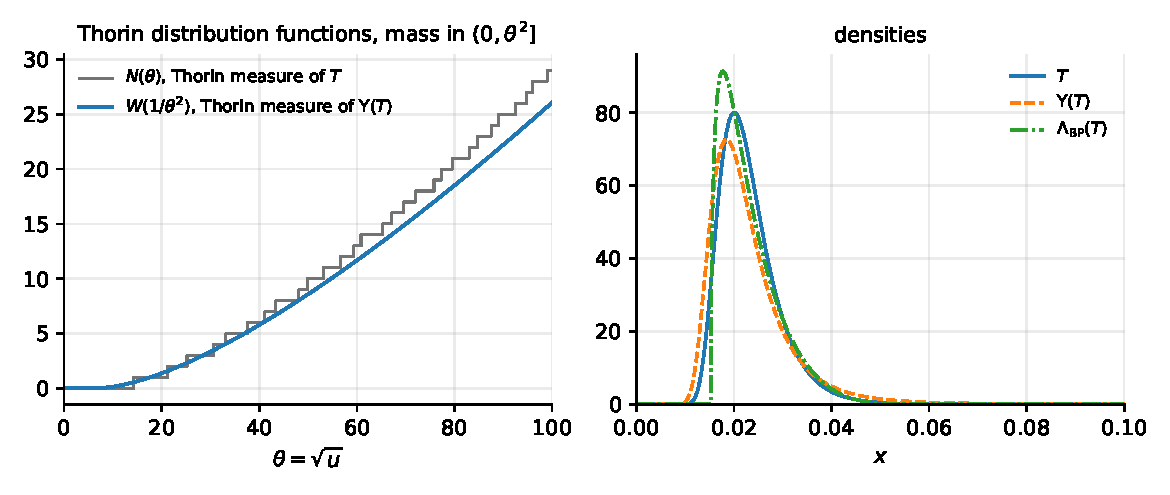
\includegraphics[width=\textwidth]{fig/wigfree_laws.pdf}
\caption{Left: the distribution function $W(\theta^{-2})$ of the Thorin measure of $\Upsilon(T)$ in the chart $\theta=\sqrt u$, against the zero count $N(\theta)$, which under RH is the distribution function of the Thorin measure of $T$ in the same chart. Right: the densities of $T$, of $\Upsilon(T)$ and of $\Lambda_{\rm BP}(T)$ on $[0,0.1]$; the last vanishes to the left of $c=0.0153$. Computed by \texttt{wigfree\_upsilon.py} and drawn by \texttt{wigfree\_plots.py}.}
\label{fig:wigfree:laws}
\end{figure}

\subsection{The semicircle as a local model for the Jacobi parameters}\label{sec:wigfree:jacobi}

Section~\ref{ch:heat} builds from the Stieltjes moments $m_0,\dots,m_{2N-1}$ the Jacobi matrix $J_N$ of the measure $\nu=\sum_ja_j^{-1}\delta_{1/a_j}$, with diagonal entries $\alpha_1,\dots,\alpha_N$ and positive off diagonal entries $\beta_1,\dots,\beta_{N-1}$, the recurrence coefficients of the orthogonal polynomials of $\nu$, computed from the Taylor coefficients of $\Xi$ at the centre alone.

For constant parameters $\alpha_n=\alpha$ and $\beta_n=\beta$ the Jacobi matrix is $\alpha+\beta(S+S^*)$ on $\ell^2(\{0,1,2,\dots\})$, with $S$ the unilateral shift, and the spectral measure of its first basis vector is the semicircle law on $[\alpha-2\beta,\alpha+2\beta]$. The $N\times N$ truncations have the eigenvalues $\alpha+2\beta\cos(\pi k/(N+1))$, $1\le k\le N$, whose distribution tends to the arcsine law with density $\big(\pi\sqrt{4\beta^2-(x-\alpha)^2}\big)^{-1}$ on the same interval, the density of states. If the parameters vary slowly, the eigenvalues are counted by integrating local arcsine laws over the rows. For recurrence coefficients that vary on the scale of the matrix size, $\alpha_{n,N}\to a(n/N)$ and $\beta_{n,N}\to b(n/N)$, this is the theorem of Kuijlaars and Van Assche \cite{KVA99}: the zero distribution of the orthogonal polynomials tends to $\int_0^1\omega_{[a(t)-2b(t),a(t)+2b(t)]}\,dt$, with $\omega_{[A,B]}$ the arcsine law on $[A,B]$. The parameters of $\nu$ decrease to zero with no such scaling, and the count needed below is that of the largest eigenvalues, an edge statement; for $\nu$ the local model is a heuristic. Since $\nu$ has its atoms in $(0,\gamma_1^{-2}]$ and accumulates only at the origin, the local interval $[\alpha_n-2\beta_n,\alpha_n+2\beta_n]$ should reach down to zero, which suggests $\alpha_n\approx2\beta_n$. Write $L(n)=\alpha_n+2\beta_n$ for its right end, taken to decrease in $n$, and $n(L)$ for the inverse function.

The eigenvalues of $J_N$ above a level $x>0$ approximate the atoms $1/\gamma_j^2$ above $x$, of which there are $N(x^{-1/2})$. In the local model row $n$ contributes the mass $\frac2\pi\arccos\sqrt{x/L(n)}$ of the arcsine law on $[0,L(n)]$ above $x$, and nothing when $x\ge L(n)$, so that
\begin{equation}\label{eq:wigfree:count}
N\big(x^{-1/2}\big)=\int_0^\infty\frac2\pi\arccos\sqrt{x/L(n)}_{\,+}\,dn=\frac1\pi\int_x^\infty n(L)\,\frac{\sqrt x\,dL}{L\sqrt{L-x}},
\end{equation}
the second form by an integration by parts in $L$. With $u=1/L$ and $w=1/x$ it becomes Abel's equation
\begin{equation}\label{eq:wigfree:abeleq}
\int_0^w\frac{f(u)\,du}{\sqrt{w-u}}=\pi N(\sqrt w),\qquad f(u)=u^{-1/2}\,n(1/u).
\end{equation}

\begin{proposition}\label{prop:wigfree:abel}
Let $N$ be nondecreasing and right continuous on $[0,\infty)$, with $N=0$ on $[0,\theta_0)$ for some $\theta_0>0$. Then
\begin{equation}\label{eq:wigfree:abel}
n(L)=\int_{(0,L^{-1/2})}\frac{dN(T)}{\sqrt{1-LT^2}}
\end{equation}
gives a locally integrable solution $f$ of \eqref{eq:wigfree:abeleq}, with $N(\sqrt w)$ replaced by its left limit at the jumps of $N$, and it is the only locally integrable solution. If $dN(T)=c\,dT$ on $(0,\infty)$, then $n(L)=\frac\pi2cL^{-1/2}$, so that $L_n=(\pi c/2n)^2$, which is $\gamma_{2n/\pi}^{-2}$ for the ordinates $\gamma_k=k/c$ of that count.
\end{proposition}

\begin{proof}
For $0<a<b$ the substitution $u=1/L$ gives
\begin{align*}
\int_a^b\frac{dL}{L\sqrt{(L-a)(b-L)}}&=\int_{1/b}^{1/a}\frac{du}{\sqrt{(1-au)(bu-1)}}\\
&=\frac1{\sqrt{ab}}\int_{1/b}^{1/a}\frac{du}{\sqrt{(1/a-u)(u-1/b)}}=\frac\pi{\sqrt{ab}} .
\end{align*}
Insert \eqref{eq:wigfree:abel} in the right side of \eqref{eq:wigfree:count}, which is equivalent to \eqref{eq:wigfree:abeleq}, and exchange the integrals, all terms being positive. A point $T$ of the support of $dN$ contributes only when $T<x^{-1/2}$, through $L\in(x,T^{-2})$, and with $b=T^{-2}$ and $\sqrt{1-LT^2}=\sqrt{(b-L)/b}$ its contribution is
\[
\frac{\sqrt x}\pi\int_x^b\frac{\sqrt b\,dL}{L\sqrt{(L-x)(b-L)}}=1 .
\]
So the right side is $N$ of the open interval $(0,x^{-1/2})$, the left limit of $N$ at $x^{-1/2}$. The function $f$ is locally integrable: $n$ vanishes for $L>\theta_0^{-2}$, and for $0<a<b$, by Fubini's theorem, $\int_a^bn(L)\,dL\le\int_{(0,a^{-1/2})}dN(T)\int_0^{T^{-2}}dL/\sqrt{1-LT^2}=2\int_{(0,a^{-1/2})}T^{-2}\,dN(T)<\infty$. If $f_1$ and $f_2$ are two locally integrable solutions, $g=f_1-f_2$ satisfies $\int_0^wg(u)(w-u)^{-1/2}du=0$ for every $w$; integrating against $(y-w)^{-1/2}$ over $w\in(0,y)$ and using $\int_u^y dw/\sqrt{(y-w)(w-u)}=\pi$ gives $\pi\int_0^yg=0$ for every $y$, so $g=0$ almost everywhere. Finally $\int_0^{L^{-1/2}}c\,dT/\sqrt{1-LT^2}=cL^{-1/2}\arcsin1$.
\end{proof}

The local model therefore predicts $\alpha_n\approx2\beta_n\approx\frac12L_n$, with $n(L_n)=n$ \cite{P26wig}. For the zeros of $\xi$ we use the smooth density $dN_0(T)=(2\pi)^{-1}\log(T/2\pi)\,dT$ on $T>2\pi$, for which the substitution $T=L^{-1/2}\sin\varphi$ gives
\[
n(L)=\frac1{2\pi\sqrt L}\int_{\varphi_0}^{\pi/2}\log\frac{\sin\varphi}{2\pi\sqrt L}\,d\varphi,\qquad\sin\varphi_0=2\pi\sqrt L .
\]
As $L\to0$, $\int_0^{\pi/2}\log\sin\varphi\,d\varphi=-\frac\pi2\log2$ gives $n(L)=(4\sqrt L)^{-1}\log(1/(4\pi\sqrt L))+O(1)$, while the rule of Proposition~\ref{prop:wigfree:abel} for a linear count, applied with the ordinates of the smooth count, $N_0(\gamma_r)=r$ with $N_0(T)=(T/2\pi)\log(T/2\pi e)+\frac78$, gives $\frac12L_n=\frac12\gamma_{2n/\pi}^{-2}$ and corresponds to $n=(4\sqrt L)^{-1}\log(1/(2\pi e\sqrt L))$ to the same order. The two rules differ by a factor that tends to one only logarithmically; this is why the cruder rule $\alpha_n\approx\frac12\gamma_{2n/\pi}^{-2}$, which treats the count as linear, is off by a factor near $1.3$.

Table~\ref{tab:wigfree:jacobi} compares the computed parameters with the two rules. The program \texttt{wigfree\_jacobi.py} computes $M_0,\dots,M_{100}$ at $1000$ digits by the trapezoid rule of step $1/600$ on $[0,3.6]$, the moments $m_0,\dots,m_{99}$, and the Cholesky factorisation of $\mathcal H_{50}$. The matrix $L^{-1}[m_{i+j+1}]L^{-\top}$ is tridiagonal to $1.3\times10^{-836}$, and its entries change by at most $2.3\times10^{-429}$ relatively when the factorisation runs at $600$ digits. The first parameters are irregular, $\alpha_1,\dots,\alpha_5=(1.61,3.50,1.80,1.22,1.07)\times10^{-3}$ and $\beta_1,\dots,\beta_5=(1.91,1.15,0.697,0.554,0.498)\times10^{-3}$, and the model is meant for larger $n$. Over $17\le n\le49$ the ratio $\alpha_n/\frac12L_n$ has mean $1.033$ and standard deviation $0.060$ (range $0.940$ to $1.178$), and $2\beta_n/\frac12L_n$ has mean $1.012$ and standard deviation $0.060$ (range $0.893$ to $1.134$); the columns $\alpha_n$, $2\beta_n$, $\frac12L_n$ and these two ratios reproduce Table~6 of \cite{P26wig} to the digits shown there. Over the same range $\alpha_n/(2\beta_n)$ has mean $1.021$ and standard deviation $0.047$, and $\beta_n^2/(\alpha_n\alpha_{n+1})$, which is $\frac14$ in the local model, has mean $0.2502$ and standard deviation $0.013$ (mean $0.256$ and standard deviation $0.059$ over $1\le n\le49$). The cruder rule falls short: $\alpha_n$ and $2\beta_n$ exceed it by the factors $1.286$ and $1.26$ on average, with standard deviations $0.081$ and $0.078$.

Two cautions apply. The rule $n(L_n)=n$ and the midpoint rule $n(L_n')=n-\frac12$ differ by a shift of $n$ of order one, which the asymptotics cannot see, and they move the mean ratios by two per cent, to $1.011$ and $0.991$, within the scatter; the data do not decide between them. And the scatter itself, about six per cent, is not explained by this computation: the note attributes it to the discreteness of the zeros, which the smooth density ignores, and that remains to be tested (Problem~\ref{prob:wigfree:jacobi}). So the local semicircle model predicts the size of the Jacobi parameters to a few per cent over $17\le n\le49$ with no fitted constant, but the agreement is not a proof of an asymptotic law.

\begin{table}[htbp]
\centering\footnotesize
\setlength{\tabcolsep}{2.6pt}
\begin{tabular}{rcccccccccc}
\toprule
 & \multicolumn{3}{c}{$10^5\times$} & \multicolumn{2}{c}{ratio to $\frac12L_n$} & $10^5\times$ & \multicolumn{2}{c}{ratio to $\frac12L_n'$} & $10^5\times$ & \\
\cmidrule(lr){2-4}\cmidrule(lr){5-6}\cmidrule(lr){7-7}\cmidrule(lr){8-9}\cmidrule(lr){10-10}
$n$ & $\alpha_n$ & $2\beta_n$ & $\frac12L_n$ & $\alpha_n$ & $2\beta_n$ & $\frac12L_n'$ & $\alpha_n$ & $2\beta_n$ & $\frac12\gamma_{2n/\pi}^{-2}$ & $\frac{\beta_n^2}{\alpha_n\alpha_{n+1}}$\\
\midrule
5 & 107.3 & 99.54 & 84.84 & 1.27 & 1.17 & 94.11 & 1.14 & 1.06 & 61.8 & 0.2665\\
9 & 56.96 & 51.12 & 45.73 & 1.25 & 1.12 & 48.70 & 1.17 & 1.05 & 34.5 & 0.2548\\
13 & 30.20 & 32.52 & 30.07 & 1.00 & 1.08 & 31.48 & 0.959 & 1.03 & 23.2 & 0.2611\\
17 & 21.71 & 21.51 & 21.83 & 0.995 & 0.986 & 22.64 & 0.959 & 0.950 & 17.0 & 0.2362\\
21 & 18.50 & 16.55 & 16.82 & 1.10 & 0.983 & 17.34 & 1.07 & 0.954 & 13.3 & 0.2479\\
25 & 15.90 & 14.58 & 13.50 & 1.18 & 1.08 & 13.85 & 1.15 & 1.05 & 10.7 & 0.2588\\
29 & 11.25 & 11.45 & 11.16 & 1.01 & 1.03 & 11.41 & 0.986 & 1.00 & 8.93 & 0.2550\\
33 & 9.530 & 9.336 & 9.424 & 1.01 & 0.991 & 9.615 & 0.991 & 0.971 & 7.59 & 0.2647\\
37 & 8.704 & 8.163 & 8.101 & 1.07 & 1.01 & 8.249 & 1.06 & 0.990 & 6.56 & 0.2463\\
41 & 6.998 & 7.053 & 7.062 & 0.991 & 0.999 & 7.179 & 0.975 & 0.982 & 5.74 & 0.2618\\
45 & 6.498 & 6.150 & 6.228 & 1.04 & 0.987 & 6.323 & 1.03 & 0.973 & 5.08 & 0.2481\\
49 & 5.957 & 6.172 & 5.547 & 1.07 & 1.11 & 5.625 & 1.06 & 1.10 & 4.54 & 0.2738\\
\bottomrule
\end{tabular}
\caption{The Jacobi parameters of $\nu$ against the local semicircle model: $\alpha_n$ and $2\beta_n$; half the right end $\frac12L_n$ of the local interval from \eqref{eq:wigfree:abel} with the smooth density and $n(L_n)=n$, and the ratios to it; the same with the midpoint rule $n(L_n')=n-\frac12$; the cruder rule $\frac12\gamma_{2n/\pi}^{-2}$, with $N_0(\gamma_r)=r$; and $\beta_n^2/(\alpha_n\alpha_{n+1})$, which is $\frac14$ in the local model. Computed by \texttt{wigfree\_jacobi.py}.}
\label{tab:wigfree:jacobi}
\end{table}

\subsection{Gamma(2), Laguerre polynomials and finite free convolution}\label{sec:wigfree:gamma2}

Williams' variable \cite{Williams90} $S_2=J+J'=\sum_n\frac2{\pi^2n^2}\Gamma_n$, with independent Gamma(2) variables $\Gamma_n$, the sum of two independent copies of the hitting time $J=\sum_n\frac2{\pi^2n^2}e_n$ of Section~\ref{bp:sec:mellin}, satisfies $2\xi(s)=\E(\frac\pi2S_2)^{s/2}$ \eqref{bp:eq:bpy} \cite{BPY01}, and the RH content of this identity lies on its Mellin side (Theorem~\ref{rz:thm:bpy} and Section~\ref{sec:ch19:williams}). The cumulants of $S_2$ are $\kappa_m=2(m-1)!\,(2/\pi^2)^m\zeta(2m)$.

\begin{proposition}\label{prop:wigfree:s1}
For every complex $s$,
\begin{equation}\label{eq:wigfree:s1}
\E\Big[\Big(\frac\pi2J\Big)^{s/2}\Big]=\frac{2(1-2^{1-s})\,\xi(s)}{s-1}=s\,\pi^{-s/2}\,\Gamma\Big(\frac s2\Big)(1-2^{1-s})\,\zeta(s),
\end{equation}
the value at $s=1$ being $2\xi(1)\log2=\log2$. Equivalently $J\stackrel d=V^{-2}S_2$, with $V$ uniform on $[1,2]$ and independent of $S_2$. The function \eqref{eq:wigfree:s1} vanishes at the zeros of $\xi$ and at the points $1+2\pi ik/\log2$, $k\ne0$, of the line $\re s=1$, and, unlike the zero set of $\xi$, its zero set is not symmetric under $s\mapsto1-s$.
\end{proposition}

\begin{proof}
This is the multiplicative relation of Biane, Pitman and Yor between $J$, their $\Sigma_1$, and $S_2$, their $\Sigma_2$ \cite[Table 1 and (43) to (45)]{BPY01}; we give the computation. For $\re p<0$, $\int_0^\infty\lambda^{-p-1}e^{-\lambda x}d\lambda=\Gamma(-p)x^p$ and $\E e^{-\lambda J}=\sqrt{2\lambda}/\sinh\sqrt{2\lambda}$ give, with $r=\sqrt{2\lambda}$,
\[
\E J^p=\frac{2^{p+1}}{\Gamma(-p)}\int_0^\infty\frac{r^{-2p}}{\sinh r}\,dr=\frac{2^{p+2}(1-2^{2p-1})\,\Gamma(1-2p)\,\zeta(1-2p)}{\Gamma(-p)},
\]
by $1/\sinh r=2\sum_{k\ge0}e^{-(2k+1)r}$, which gives $\int_0^\infty r^{z-1}/\sinh r\,dr=2(1-2^{-z})\Gamma(z)\zeta(z)$ for $\re z>1$. Put $p=s/2$ with $\re s<0$. The functional equation $\zeta(1-s)=\pi^{1/2-s}\Gamma(\frac s2)\zeta(s)/\Gamma(\frac{1-s}2)$, the duplication formula $\Gamma(1-s)=2^{-s}\pi^{-1/2}\Gamma(\frac{1-s}2)\Gamma(1-\frac s2)$ and $\Gamma(1-\frac s2)/\Gamma(-\frac s2)=-\frac s2$ turn this into $\E J^{s/2}=-2^{1-s/2}s(1-2^{s-1})\pi^{-s}\Gamma(\frac s2)\zeta(s)$, and multiplying by $(\pi/2)^{s/2}$ gives \eqref{eq:wigfree:s1}. Both sides are entire, since $J$ has moments of all real orders and the zero of $1-2^{1-s}$ at $s=1$ cancels the pole of $\zeta$, so the identity holds for every $s$. Since $\E V^{-s}=\int_1^2v^{-s}dv=(1-2^{1-s})/(s-1)$, the right side is $\E V^{-s}\,\E(\frac\pi2S_2)^{s/2}$. The factor $1-2^{1-s}$ vanishes exactly at $1+2\pi ik/\log2$; on the line $\re s=0$, the image of $\re s=1$ under $s\mapsto1-s$, it equals $-1$ at the corresponding points $2\pi ik/\log2$ and $\xi$ has no zeros, so the zero set is not symmetric.
\end{proof}

The elementary factor $(1-2^{1-s})/(s-1)$ adds zeros on the line $\re s=1$, the first at height $2\pi/\log2=9.0647$, the zeros of the alternating zeta function that Section~\ref{wr:sec:salem} meets.

\begin{proposition}\label{prop:wigfree:wishart}
Let $z_1,z_2,\dots$ be independent standard complex Gaussian vectors in $\C^2$, with $\E z_nz_n^*=I_2$, let $c_n=2/(\pi^2n^2)$ and $W=\sum_nc_nz_nz_n^*$. Then $\operatorname{tr}W\stackrel d=S_2$, so that $2\xi(s)=\E(\frac\pi2\operatorname{tr}W)^{s/2}$, and
\[
\E\det(x-W)=x^2-2m_1x+m_1^2-m_2,\qquad m_k=\sum_nc_n^k,\quad m_1=\tfrac13,\ m_2=\tfrac2{45},
\]
with the real roots $m_1\pm\sqrt{m_2}=0.122515$ and $0.544152$. This is the finite free convolution $\boxplus_2$ of the polynomials $\E\det(x-c_nz_nz_n^*)=x(x-2c_n)$, and the mixed characteristic polynomial of Marcus, Spielman and Srivastava \cite{MSS15} of the matrices $c_nI_2$.
\end{proposition}

\begin{proof}
$|z_n|^2$ is the sum of two independent standard exponential variables, so $\operatorname{tr}W=\sum_nc_n|z_n|^2\stackrel d=S_2$. For a $2\times2$ matrix, $\det(x-W)=x^2-x\operatorname{tr}W+\det W$ and $\det W=\frac12((\operatorname{tr}W)^2-\operatorname{tr}W^2)$. Here $\E\operatorname{tr}W=2m_1$ and $\E(\operatorname{tr}W)^2=\operatorname{Var}S_2+(\E S_2)^2=2m_2+4m_1^2$, while $\E\operatorname{tr}W^2=\sum_{n,k}c_nc_k\E|z_n^*z_k|^2=6m_2+2(m_1^2-m_2)$, since $\E|z_n|^4=6$ and $\E|z_n^*z_k|^2=\operatorname{tr}(I_2I_2)=2$ for $n\ne k$. Hence $\E\det W=m_1^2-m_2$. The terms $c_nz_nz_n^*$ are independent and unitarily invariant in law, with $\E\det(x-c_nz_nz_n^*)=x^2-2c_nx$, so by \cite[Theorem 1.2]{MSS22} and bilinearity the expected characteristic polynomial of a finite partial sum is the $\boxplus_2$ convolution of these polynomials; with the coefficient formula of $\boxplus_2$, adding $x(x-2c)$ to a polynomial $x^2-Ax+B$ gives $x^2-(A+2c)x+B+Ac$, so the constant term is $2\sum_{n<k}c_nc_k=m_1^2-m_2$ in the limit.
\end{proof}

The reading of the exponent two of $(\sqrt{2\lambda}/\sinh\sqrt{2\lambda})^2$ as the size of the matrix is special to the sinh family of \cite{BPY01}.

In the normalisation of \cite{MSS22} write a polynomial of degree $d$ as $p(x)=\sum_k(-1)^k\binom dke_kx^{d-k}$; the multiplicative convolution $\boxtimes_d$ multiplies the normalised coefficients, $e_k(p\boxtimes_dq)=e_k(p)e_k(q)$ \cite[Definition 1.4]{MSS22}, and by Szeg\H{o}'s theorem it preserves the property of having only nonnegative roots \cite[Theorem 1.6]{MSS22}.

\begin{lemma}\label{lem:wigfree:laguerre}
Let $a>0$ and $(a)_k=a(a+1)\cdots(a+k-1)$.
\begin{enumerate}
\item[(i)] The reversed Laguerre polynomial $q_a(x)=x^dL_d^{(a-1)}(1/x)$ has $d$ positive simple roots and normalised coefficients $e_k=e_0/(a)_k$, $e_0=\Gamma(d+a)/(d!\,\Gamma(a))$. Hence $p\boxtimes_d(q_a/e_0)$ has the normalised coefficients $e_k(p)/(a)_k$, and it has only real roots whenever the roots of $p$ are real and of one sign.
\item[(ii)] $\{1/(a)_k\}_{k\ge0}$ is a multiplier sequence: the function
\[
\sum_k\frac{x^k}{k!\,(a)_k}=\Gamma(a)x^{(1-a)/2}I_{a-1}(2\sqrt x)
\]
is entire of order $\frac12$ with only real negative zeros, at $-j_{a-1,m}^2/4$.
\item[(iii)] A density $f$ on $(0,\infty)$ is a scale mixture of Gamma$(a)$ densities if and only if $x^{1-a}f(x)$ is completely monotone; for $a=2$, if and only if $f(x)/x$ is.
\end{enumerate}
\end{lemma}

\begin{proof}
(i) By \cite[(18.5.12)]{DLMF},
\[
x^dL_d^{(a-1)}(1/x)=\sum_k(-1)^k\binom{d+a-1}{d-k}\frac{x^{d-k}}{k!},
\]
and $\binom{d+a-1}{d-k}/(k!\binom dk)=\Gamma(d+a)/(d!\,\Gamma(k+a))$, which is $e_0/(a)_k$. The zeros of $L_d^{(a-1)}$ are positive and simple, those of an orthogonal polynomial for the weight $x^{a-1}e^{-x}$ on $(0,\infty)$ \cite[Section 18.2(vi)]{DLMF}, and the roots of $q_a$ are their reciprocals. The statement on $\boxtimes_d$ is Szeg\H{o}'s theorem for roots of one sign; for nonpositive roots apply it to $(-1)^dp(-x)$, whose normalised coefficients are $(-1)^ke_k(p)$. (ii) The series is that of the modified Bessel function \cite[(10.25.2)]{DLMF}. For $x=-y^2/4<0$ it equals $\Gamma(a)(y/2)^{1-a}J_{a-1}(y)$, and for $a-1>-1$ the zeros of $J_{a-1}(y)/y^{a-1}$ are real \cite[Section 10.21(i)]{DLMF}. A real entire function of order less than one with only real zeros is in the Laguerre P\'olya class, and by the theorem of P\'olya and Schur \cite{PS14} a sequence whose exponential generating function is in that class with coefficients of one sign is a multiplier sequence. (iii) $f(x)=\int_0^\infty\theta^{-a}x^{a-1}e^{-x/\theta}\,\varpi(d\theta)/\Gamma(a)$ says that $x^{1-a}f(x)$ is the Laplace transform of a positive measure in the variable $1/\theta$; conversely Bernstein's theorem writes a completely monotone $x^{1-a}f(x)$ in this form.
\end{proof}

Let $X$ be the P\'olya variable, with density $p=\Phi/\Xi(0)$ for the kernel $\Phi$ of \eqref{eq:ch2:Phi} and moment generating function $\E e^{sX}=G(s^2)$ \eqref{eq:ch2:mgf}, and write $G(u)=\sum_kb_ku^k$, so that $b_k=\E X^{2k}/(2k)!=M_k/((2k)!\,M_0)$ with $M_k=\int_\R v^{2k}\Phi(v)\,dv$, as in Sections~\ref{ch:heat} and~\ref{fm:sec:polyanec}.

\begin{proposition}\label{prop:wigfree:peel}
For $a>0$ let $G_a(u)=\sum_kb_ku^k/(a)_k$. If RH holds, then for every $a>0$ the function $G_a$ is in the Laguerre P\'olya class with only real negative zeros, and all its Jensen polynomials $\sum_{i=0}^d\binom di(n+i)!\,b_{n+i}x^i/(a)_{n+i}$, $d,n\ge0$, have only real negative zeros. Multiplying the coefficients by $(a)_k$ instead does not preserve real zeros: it turns $(1+u)^2=1+2u+u^2$ into $1+2au+a(a+1)u^2$, whose discriminant is $-4a<0$.
\end{proposition}

\begin{proof}
Under RH, $G(u)=\prod_j(1+u/\gamma_j^2)$ with $\sum_j\gamma_j^{-2}<\infty$, so $G$ is in the Laguerre P\'olya class, and by P\'olya's theorem its Jensen polynomials $J_{d,n}(x)=\sum_i\binom di(n+i)!\,b_{n+i}x^i$ of Section~\ref{fm:sec:polyanec} have only real zeros. Since $(a)_{n+i}=(a)_n(a+n)_i$, the Jensen polynomial of $G_a$ of degree $d$ and shift $n$ is $1/(a)_n$ times the image of $J_{d,n}$ under the multiplier sequence $\{1/(a+n)_i\}_i$ of Lemma~\ref{lem:wigfree:laguerre}(ii), so it has only real zeros, negative because its coefficients are positive. For $n=0$, $\binom di\,i!\,d^{-i}\to1$ gives $\sum_i\binom di\,i!\,b_ix^i/((a)_id^i)\to G_a(x)$ uniformly on compact sets as $d\to\infty$, so by Hurwitz's theorem $G_a$ has only real negative zeros; since $(a)_k\ge a(k-1)!$, $G_a$ has order at most $\frac13$, and it is in the Laguerre P\'olya class. The example is a direct computation.
\end{proof}

In terms of Lemma~\ref{lem:wigfree:laguerre}(i), dividing the normalised coefficients by $(a)_k$ is the multiplicative convolution with $q_a/e_0$, so peeling a Gamma($a$) layer, the operation that would pass from the moments of a Gamma($a$) scale mixture to those of its mixing law, keeps zeros real, while the inverse operation can destroy them. The note calls the peeling a free Poisson operation. The example does not show that no argument could pass from real zeros of some $G_a$ to real zeros of $G$, as the note puts it.

Lemma~\ref{lem:wigfree:laguerre}(iii) makes the Gamma(2) mixture route of \cite[Section 12.6]{P26}, which Section~\ref{sec:ch19:williams} recalls as excluded, a statement about complete monotonicity.

\begin{theorem}\label{thm:wigfree:nomix}
For no $a>0$ is $|X|$, $X^2$ or $S_2$ a scale mixture of Gamma$(a)$ laws.
\end{theorem}

\begin{proof}
By Lemma~\ref{lem:wigfree:laguerre}(iii) a mixture would make $g(x)=x^{1-a}f(x)$ completely monotone, with $f$ the density. A completely monotone $g\not\equiv0$ is positive and log convex, so $g(x)\ge g(1)\exp\big((x-1)g'(1)/g(1)\big)$ for $x\ge1$: it decays at most exponentially. For $v\ge0$, dropping the negative terms of \eqref{eq:ch2:Phi} and using $e^{2v}\ge1$ gives
\[
\Phi(v)\le4\pi^2e^{9v/2}\exp(-\pi e^{2v})\sum_{n\ge1}n^4e^{-\pi(n^2-1)},
\]
a constant multiple of $e^{9v/2}\exp(-\pi e^{2v})$. The densities of $|X|$ and $X^2$ are $2\Phi(v)/\Xi(0)$ and $\Phi(\sqrt w)/(\Xi(0)\sqrt w)$, so $v^{1-a}\Phi(v)$ and $w^{1/2-a}\Phi(\sqrt w)$ would have to be completely monotone, and both decay faster than any exponential. For $S_2$ the obstruction is at the origin. By Chebyshev's inequality in exponential form, for $\lambda>0$, $\Pr(S_2\le x)\le e^{\lambda x}\E e^{-\lambda S_2}=e^{\lambda x}\big(\sqrt{2\lambda}/\sinh\sqrt{2\lambda}\big)^2$, and $\lambda=2/x^2$ gives
\[
\Pr(S_2\le x)\le\frac{16\,e^{-2/x}}{x^2(1-e^{-4/x})^2}\le17\,x^{-2}e^{-2/x},\qquad0<x\le1 .
\]
A mixture would give, $g$ being nonincreasing and $g(1)>0$, $f(x)\ge g(1)x^{a-1}$ and $\Pr(S_2\le x)\ge g(1)x^a/a$ for $0<x\le1$, which is impossible as $x\downarrow0$.
\end{proof}

The Hankel test sees the failure at low order. If $Y=\Theta\,\Gamma$ with $\Gamma$ a Gamma$(a)$ variable independent of $\Theta\ge0$, then $\E Y^k=(a)_k\E\Theta^k$, so $\mu_k=\E Y^k/(a)_k$ must be a Stieltjes moment sequence, and both $[\mu_{i+j}]_{i,j<N}$ and $[\mu_{i+j+1}]_{i,j<N}$ must be positive semidefinite for every $N$. Table~\ref{tab:wigfree:hankel} gives the least order $N$ at which each fails to be positive definite, by Cholesky factorisation at $400$ digits, with the same orders at $250$. The moments of $X^2$ are $M_k/M_0$; those of $|X|$ come from a tanh sinh rule, since odd powers of $|v|$ are not smooth at the origin; those of $S_2$ follow from its cumulants. The table of \cite{P26wig} is the Hamburger row, the first matrix alone.

\begin{table}[htbp]
\centering\footnotesize
\setlength{\tabcolsep}{4pt}
\begin{tabular}{lccccccccccc}
\toprule
$a$ & $\frac12$ & $1$ & $\frac32$ & $2$ & $\frac52$ & $3$ & $4$ & $6$ & $8$ & $12$ & $20$\\
\midrule
$|X|$, Stieltjes & 2 & 2 & 2 & 2 & 2 & 3 & 3 & 3 & 4 & 4 & 5\\
$|X|$, Hamburger & 2 & 2 & 2 & 3 & 3 & 3 & 3 & 4 & 4 & 5 & 6\\
$X^2$, Stieltjes & 2 & 3 & 3 & 4 & 4 & 4 & 5 & 5 & 6 & 7 & 9\\
$X^2$, Hamburger & 2 & 3 & 4 & 4 & 4 & 5 & 5 & 6 & 6 & 7 & 9\\
$S_2$, both & 2 & 2 & 2 & 2 & 2 & 2 & 2 & 3 & 4 & 6 & 12\\
\bottomrule
\end{tabular}
\caption{The first order $N$ at which the moments $\mu_k=\E Y^k/(a)_k$ fail the Hankel test for a Gamma$(a)$ scale mixture, for $Y=|X|$, $X^2$ and $S_2$: the Hamburger test uses $[\mu_{i+j}]_{i,j<N}$ alone, the Stieltjes test also $[\mu_{i+j+1}]_{i,j<N}$. Computed by \texttt{wigfree\_gamma2.py}.}
\label{tab:wigfree:hankel}
\end{table}

The theorem also settles which tool applies. Kristiansen proved Steutel's conjecture that scale mixtures of Gamma(2) laws are infinitely divisible \cite{Kristiansen94}; since $x^{\alpha-2}e^{-x}$ is completely monotone for $\alpha\le2$, Lemma~\ref{lem:wigfree:laguerre}(iii) makes Gamma$(\alpha)$ itself a scale mixture of Gamma(2) laws, and the theorem covers scale mixtures of Gamma$(\alpha)$ laws for every $\alpha\le2$. By Theorem~\ref{thm:wigfree:nomix} it cannot be applied to $|X|$, $X^2$ or $S_2$. The Gamma(2) structure that is true is Williams' convolution, a GGC and hence infinitely divisible directly.

\subsection{The heat flow and finite free convolution}\label{sec:wigfree:heat}

Remark~\ref{rem:wigbiane:direction} identifies the forward heat flow on polynomials with finite free convolution by a Hermite polynomial and, as the degree grows, with free convolution by a semicircle law. The time is the variance of the semicircle law. For a real polynomial $p$ of degree $d\ge2$ write $p_t=e^{-(t/2)D^2}p$, a finite sum, and
\[
q_t(x)=e^{-(t/2)D^2}x^d=t^{d/2}H_d\big(x/\sqrt t\big),\qquad t>0,
\]
with $q_0=x^d$ and $H_d=e^{-D^2/2}x^d$ the Hermite polynomial of Remark~\ref{rem:wigbiane:direction}, whose zeros are real. The time $t$ is twice the time of Section~\ref{sec:ch21:flow}, where $\partial_tH_t=-\partial_z^2H_t$.

\begin{proposition}\label{prop:wigfree:heat}
Let $p$ be a real polynomial of degree $d\ge2$ and $s,t\ge0$.
\begin{enumerate}
\item[(i)] $p_t=p\boxplus_dq_t$.
\item[(ii)] $q_s\boxplus_dq_t=q_{s+t}$.
\item[(iii)] If $p$ has only real roots, then so has $p_t$, and the largest root of $p_t$ is at most the largest root of $p$ plus $\sqrt t\,h_d$, where $h_d$ is the largest zero of $H_d$.
\item[(iv)] While the roots $z_1(t),\dots,z_d(t)$ of $p_t$ are simple, $\dot z_k=\sum_{j\ne k}(z_k-z_j)^{-1}$.
\end{enumerate}
\end{proposition}

\begin{proof}
(i) In operator form, $p\boxplus_dq=\hat p(D)\hat q(D)x^d$ when $p=\hat p(D)x^d$ and $q=\hat q(D)x^d$ \cite[Definition 1.1 and (2)]{MSS22}. For $q=q_t$ the operator $\hat q(D)$ acts on polynomials of degree at most $d$ as $e^{-(t/2)D^2}$, and operators in $D$ commute, so $p\boxplus_dq_t=e^{-(t/2)D^2}\hat p(D)x^d=p_t$. (ii) is (i) for $p=q_s$, since $e^{-(t/2)D^2}e^{-(s/2)D^2}=e^{-((s+t)/2)D^2}$; it is the identity $a^dH_d(x/a)\boxplus_db^dH_d(x/b)=c^dH_d(x/c)$, $c^2=a^2+b^2$, of \cite[Section 1.2]{MSS22}. (iii) The roots of $q_t$ are $\sqrt t$ times those of $H_d$, and by Walsh's theorem \cite[Theorem 1.3]{MSS22} the convolution $p\boxplus_dq$ of two polynomials of degree $d$ with only real roots has only real roots, the largest at most the sum of the largest roots of $p$ and $q$. (iv) Differentiate $p_t(z_k(t))=0$ in $t$ and use $\partial_tp_t=-\frac12p_t''$: $\dot z_k=\frac12p_t''(z_k)/p_t'(z_k)$. Writing $p_t=(x-z_k)r$ gives $p_t'(z_k)=r(z_k)$ and $p_t''(z_k)=2r'(z_k)$, so that $\dot z_k=r'(z_k)/r(z_k)=\sum_{j\ne k}(z_k-z_j)^{-1}$.
\end{proof}

For a conjugate pair $x\pm iy$, $y>0$, the partner contributes $-1/(2y)$ to $\dot y$, and each real root $r$ contributes $\im(x+iy-r)^{-1}=-y/((x-r)^2+y^2)<0$: the pair is drawn to the axis by its partner and pulled further by every real root. On its own, $(x-1)^2+0.64$ becomes $(x-1)^2+0.64-t$, which reaches the axis at $t=0.64$. The example of the note adds four real roots,
\[
p(x)=(x+3)(x+1)\big(x-\tfrac12\big)(x-2)\big((x-1)^2+0.64\big).
\]
The discriminant of $p_t$ in $x$ is a polynomial of degree $15$ in $t$ whose only root in $(0,2)$ is $t^*=0.3203291143987806$. Before $t^*$ the roots are distinct, so the pair stays off the axis, and since $p_t=e^{-((t-t^*)/2)D^2}p_{t^*}$ for $t>t^*$, part (iii) keeps all roots real afterwards: the pair meets the axis at $t^*$, at the point $1.25743$, in about half the time it needs on its own. The program \texttt{wigfree\_heat.py} computes the discriminant exactly.

\begin{figure}[htbp]
\centering
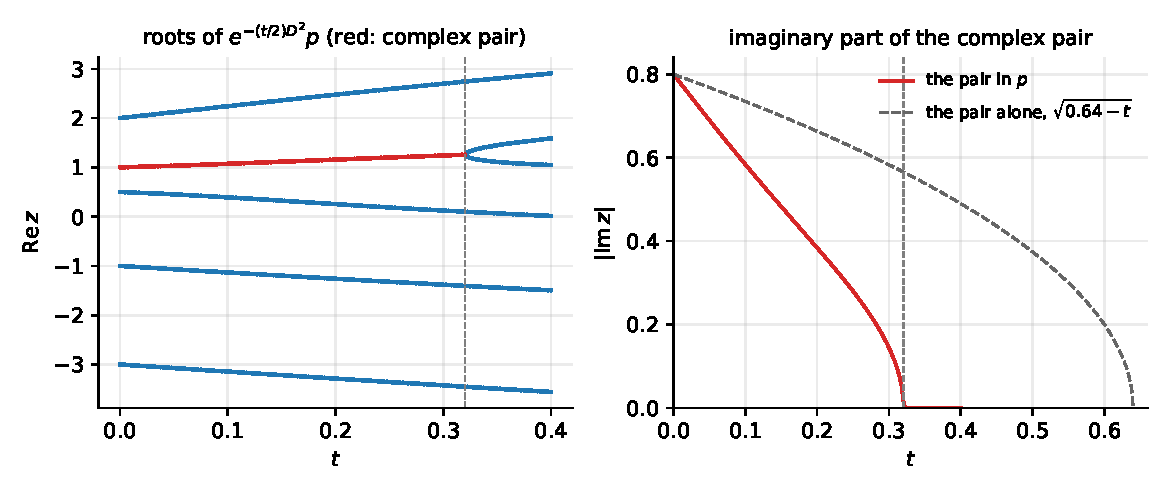
\includegraphics[width=\textwidth]{fig/wigfree_heat.pdf}
\caption{The flow $e^{-(t/2)D^2}p$ for $p$ with the roots $-3$, $-1$, $\frac12$, $2$ and $1\pm0.8i$. Left: the real parts of the six roots for $0\le t\le0.4$; the complex pair has one real part until it meets the axis at $t^*=0.3203$ (dashed), where its two roots split. Right: the imaginary part of the pair, against $\sqrt{0.64-t}$ for the pair on its own, which reaches the axis at $t=0.64$. Computed by \texttt{wigfree\_heat.py} and drawn by \texttt{wigfree\_plots.py}.}
\label{fig:wigfree:heat}
\end{figure}

The Hermite polynomial is the finite free counterpart of the semicircle law: $H_d$ is the expected characteristic polynomial of a symmetric Gaussian matrix \cite[Section 1.2]{MSS22}, and the roots of $H_d(\sqrt d\,x)$, the roots of $q_{1/d}$, are close to the quantiles $x_k$ of $\sigma_1$ given by $\sigma_1([-2,x_k])=(k-\frac12)/d$. The largest deviation from the quantiles is at the edge, and its products with $d^{2/3}$, from $0.3906$ to $0.4962$ for $d=20$ to $320$, grow slowly, as they should at the edge scale $d^{-2/3}$ of the extreme zeros. In the limit $d\to\infty$ finite free convolution becomes free convolution \cite{AP18}, \cite[Section 1.2]{MSS22}: if the root distributions of polynomials $p_d$ with only real roots tend to a law $\mu$ in moments, those of $p_d\boxplus_dq_{t/d}$ tend to $\mu\boxplus\sigma_t$.

For $H_t$ the identification is a heuristic. The motion of the zeros is the same, up to the factor two in the time (Section~\ref{sec:ch21:flow}), but $H_t$ has infinitely many zeros, with a density that grows logarithmically, while the limit theorem concerns the distribution of all $d$ roots of a polynomial after scaling; for $H_t$ it would have to be applied to windows of zeros, with the zeros outside a window acting as an external field, and no theorem of this kind is known. De Bruijn's theorem that real zeros of $H_t$ stay real forward in time \cite{deBruijn} is the counterpart of (iii), proved directly. In Thorin terms the forward flow is the path of clocks $R_t$ of Section~\ref{sec:ch21:flow}, in the time of $H_t$ (Theorem~\ref{rz:thm:dbn}).

The Jensen polynomials of Section~\ref{fm:sec:polyanec} meet the Hermite polynomials directly. Griffin, Ono, Rolen and Zagier proved that for each degree $d$ the Jensen polynomials $J_{d,n}$, after an affine change of variable and a normalisation depending on $n$, tend to the Hermite polynomial of degree $d$ as $n\to\infty$, and this is how they obtain real zeros for all large shifts \cite{GORZ19}. In the language of this subsection the Jensen polynomials of large shift are asymptotically finite free Gaussian; Problem~\ref{prob:wigfree:jensen} asks for an exact finite free structure at every shift.

These limits see the zeros only through their distribution. Moving $o(d)$ of the $d$ roots changes no limit law, so a single nonreal pair is invisible to free convolution limits, and these limits cannot decide RH by themselves \cite{P26wig}.
